%% 
%% Copyright 2025 Ryan Cardenas
%% 
%% This file contains the source code for my thesis project as part of the WQU 
%% Capstone 690 course at WorldQuant University. It is based on the Elsevier
%% template, which can be found at: 
%% https://www.elsevier.com/researcher/author/policies-and-guidelines/latex-instructions
%% 
%% This document is not intended for distribution outside of the WorldQuant University
%% Capstone 690 course without permission from the author.
%%


\documentclass[final,3p,times,authoryear]{elsarticle}

%% The amssymb package provides various useful mathematical symbols
\usepackage{amssymb}
%% The amsmath package provides various useful equation environments.
\usepackage{amsmath}
%% For importing images
\usepackage{graphicx}
\graphicspath{ {./images/} }

\usepackage{caption}

\journal{WorldQuant University Capstone Course 690}

\begin{document}


\begin{frontmatter}

    \title{Empirical Comparison of Probability Risk Premia in S\&P 500 Index Options\tnoteref{t1}}
    \tnotetext[t1]{November 18, 2025 - This document is submitted to the WorldQuant University Capstone 690 course as a requirement for the M.Sc. in Financial Engineering.} 

    \author{Ryan Cardenas}
    \ead{cardenasr913@gmail.com}
    \affiliation{organization={WorldQuant University}}

  
    \begin{abstract}
    We compared risk-neutral probabilities and realized probabilities for SPX options over a 15-year window. Using two different methods for obtaining the risk-free rate and continuous dividend yield inputs to the Black-Scholes-Merton equations, we found that call prices have historically underestimated real-world probabilities and put prices have historically overestimated real-world probabilities to an extent that is not fully explained by the long-term market trend.
    \end{abstract}

    %% Keywords
    \begin{keyword} %% keywords here, in the form: keyword \sep keyword
      risk-neutral probability \sep European options \sep treasury yield term structure
    \end{keyword}
    
\end{frontmatter}


%% Use \section commands to start a section
\section{Introduction}
  Risk-neutral probabilities have fascinated researchers in financial engineering ever since \citet{black_pricing_1973} first published their risk-neutral method for pricing European options. In the years that followed, \citet{ross_arbitrage_1976} introduced the concepts of state-prices and stochastic discount factors (also called "pricing kernels"), which represent the risk-neutral value of future payoff states and the weight investors apply to those states, respectively. \citet{breeden_prices_1978} then presented a model-free method for extracting risk-neutral probability densities using call option prices across different strikes, enabling a generation of researchers to explore empirical methods for deriving insights from options prices.

  One such insight is depicted in \citet{figlewski_risk-neutral_2018}: when compared against a lognormal distribution with volatility derived from a weighted combination of historical volatility and the VIX, the options-implied risk-neutral probability distribution displays a noticeable negative skew and body that is shifted to the right. The ratio of the two distributions discounted by the risk-free rate produces a pricing kernel that places heavy weight on lower states with a temporary "hill" at intermediate higher states before continuing to slope downward. This common and well-documented behavior contrasts starkly with the downward-sloping monotonicity predicted by utility theory, producing a conundrum that \citet{jackwerth_option-implied_2004} calls the "pricing kernel puzzle".

  At the same time, another commonly observed phenomenon known as the "volatility smile" reveals that options with different strikes generate different implied volatilities, suggesting that the market incorporates additional risk premia for strikes far from the underlying. Are these strike-dependent premia due to market participants anticipating higher real-world probabilities for these future states, or are they the result of asymetrical, wealth-dependent aversion to large losses and preference toward modest gains? \citet{jackwerth_option-implied_2004}, \citet{figlewski_risk-neutral_2018}, \citet{shiratsuka_information_2001}, and \citet{anagnou_relation_2002} all indicate that risk-neutral probabilities are poor predictors of real-world probabilities while acknowledging the difficulties in ruling them out as predictors. Regardless of its source, the discrepancy between implied volatility and realized volatility--the so-called "volatility risk premium"--suggests that market participants are influenced by more than just real-world probabilities.

  This all begs the questions: how do risk-neutral probabilities generally compare to their real-world counterparts? Additionally, how does this relationship--the \textit{probability} risk premium--vary across different strikes or moneyness levels? To address these two questions, we looked to the past.

\section{Methodology}
  \label{methodology}
  
  \subsection{General Index and Options Data}
    We downloaded historical, raw (non-adjusted) OHLC data recorded at daily intervals for the S\&P 500 index (SPX) from Yahoo Finance. In computing option contract payoffs at expiry, we used SPX prices at market open for standard options, which are AM-settled on the third Friday of each month. For all non-standard "weekly" options, which are PM-settled, we used SPX prices at market close.

    We obtained 15 years of end-of-day SPX options data (2010 through 2024) from \citet{firstrate_data_historical_nodate}, totaling over 30 million rows--one for each contract-day. This data includes trade date, expiry date, strike, bid price, and ask price. Although FirstRate Data also provides options Greeks, the underlying model assumptions are not available, so we recomputed the relevant values ourselves using the Black-Scholes-Merton equations shown below:

    \begin{align}
        &d_1 = \frac{
          \ln{\left(\frac{S}{K}\right)} + (r - q + 0.5 \sigma^2) T
        }{
          \sigma \sqrt{T}
        } \\
        &d_2 = d_1 - \sigma \sqrt{T}
    \end{align}

    For Calls:
    \begin{align}
      &C = S {\rm e}^{-q T} F(d_1) - K {\rm e}^{-r T} F(d_2) \\
      &\Delta_C = {\rm e}^{-q T} F(d_1) \\
      &Q_C(\text{ITM}) = F(d_2) \label{eq:q_measure_c}
    \end{align}

    For Puts:
    \begin{align}
      &P = K {\rm e}^{-r T} F(-d_2) - S {\rm e}^{-q T} F(d_1) \\
      &\Delta_P = -{\rm e}^{-q T} F(-d_1) \\
      &Q_P(\text{ITM}) = F(-d_2) \label{eq:q_measure_p}
    \end{align}

    Where $F(\cdot)$ is the normal cumulative distribution function, $S$ is the underlying price at entry, $K$ is the strike price, $r$ is the annualized risk-free rate, $q$ is the annualized continuous dividend yield, $T$ is the years to maturity (e.g. $T=\frac{1}{12}$ for a one-month maturity), and $\sigma$ is the volatility of the underlying geometric Brownian motion process that generates $S$. The symbol $\Delta$ represents the options delta--the rate of change of options price with respect to underlying price. $Q(\text{ITM})$ (or simply $Q$) represents the risk-neutral probability of expiring in-the-money and is different from the real-life probability $P$, which is easy to compute only in hindsight.

    Our approach to computing Q-probabilities relied on extracting implied volatilities from options prices. Doing so, however, required two economic inputs: the risk-free rate and the dividend yield. To derive these inputs, we explored two methods.

  \subsection{The FRED/Shiller Method}
    The Federal Reserve Bank of St. Louis \citep{fred_federal_2025} provides daily treasury yield data, which we downloaded via the FRED API in Python. Specifically, we obtained market yields on U.S. treasury securities quoted on an investment basis for 1-month, 3-month, 6-month, 1-year, 2-year, 3-year, 5-year, 7-year, 10-year, 20-year, and 30-year maturities. To represent overnight yields, we concatenated the Effective Federal Funds Rate (EFFR) with the Secured Overnight Financing Rate (SOFR). SOFR data is only available from 2018 onward; for all earlier dates, we used EFFR as the overnight rate. We then applied a cublic spline interpolation to the treasury yields as a function of years-to-maturity, producing a term structure useful for modeling risk-free rates for options contracts with various expirations. Figure \ref{fig:yield_1} shows an example yield curve with a one-year horizon constructed from data on November 1, 2025. Figure \ref{fig:yield_30} shows the same yield curve with a 30-year horizon.

    \begin{figure}[btp]
      \centering
      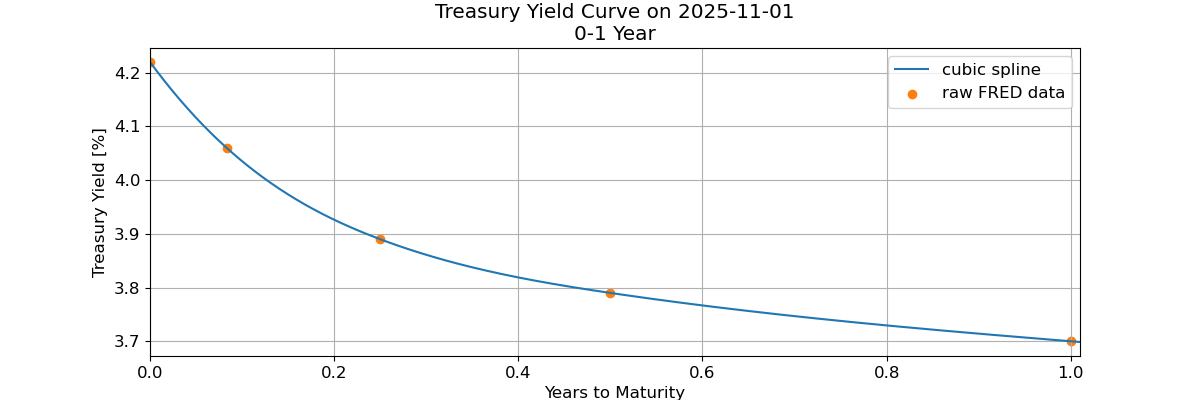
\includegraphics[width=1\textwidth]{yield_curve_1y_on_2025-11-01.png}
      \captionsetup{width=.5\linewidth}
      \caption{Term structure on November 1, 2025, constructued via cubic spline interpolation. On this particular day, treasury yields varied from 3.7\% to just over 4.2\%.}
      \label{fig:yield_1}
    \end{figure}

    \begin{figure}[btp]
      \centering
      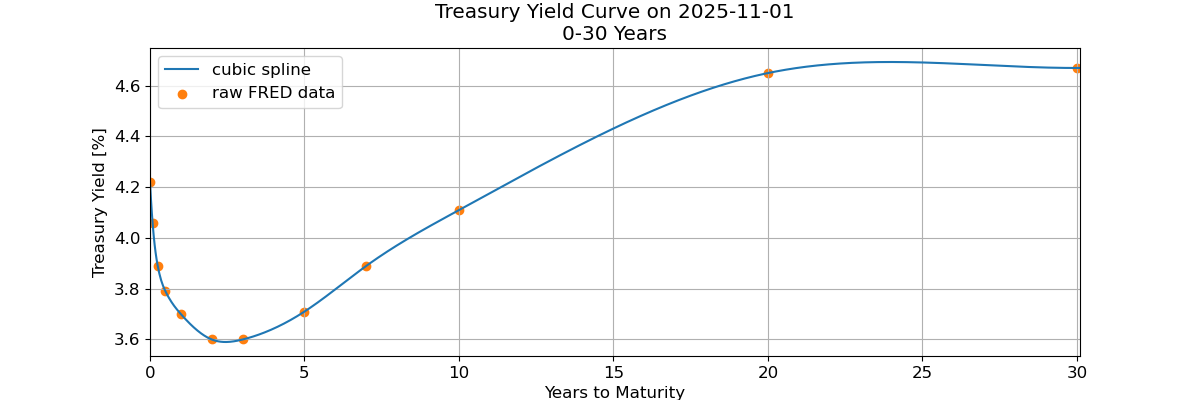
\includegraphics[width=1\textwidth]{yield_curve_30y_on_2025-11-01.png}
      \captionsetup{width=.5\linewidth}
      \caption{The same term structure as in Fig. \ref{fig:yield_1}, but zoomed out to view the full 30-year horizon. At this scale, we see the full range of yields from 3.6\% to 4.7\%.}
      \label{fig:yield_30}
    \end{figure}

    To model dividend yields, we accessed S\&P 500 quarterly dividend data curated by Yale Professor Robert J. Shiller \citep{shiller_shiller_2025}. These dividend yields average over a trailing 12-month period. Shiller retroactively interpolates this data to monthly intervals, but in live trading scenarios aggregated dividend data is only available on a quarterly basis. For this reason, we forward-filled the 12-month yields from the beginning of each fiscal quarter (March, June, September, and December) onto each trading day.

  \subsection{Shimko's Method}
    Treasury yields and continuous dividend yields provide an idealized model for pricing options, but real-world options prices account for costs of carry, discrete dividends, and various sources of trading friction. To address this reality, \citet{shimko_bounds_1993} demonstrated an empirical approach using put-call parity to derive the market-implied interest rates and dividend yields. In particular, put-call parity can be expressed as:

    \begin{align}
      C - P &= S {\rm e}^{-q T} - K {\rm e}^{-r T}
    \end{align}

    Formulating this as a linear regression problem:

    \begin{align}
      y &= m x + b \notag \\
      C - P &= m K + b
    \end{align}

    Where $m = -{\rm e}^{-r T}$ and $b = S {\rm e}^{-q T}$. For any given trade date and expiry date, the $C - P$ values observable at different strikes $K$ form a downward sloping line, the parameters of which allow us to solve for $r$ and $q$.
    
  \subsection{Computing Q-Measures and P-Measures}
    The FRED/Shiller and Shimko methods provided the $r$ and $q$ inputs to the Black-Scholes-Merton equations, making it possible to reverse-engineer the volatility parameter $\sigma$ that best reproduces observed options prices. To perform this reverse-engineering, we used Scipy's implementation of Brent's method for finding roots, with the Newton-Raphson method as a backup in case of non-convergence. We then dropped any rows where both root-finding algorithms failed to converge on a solution for $\sigma$.

    One challenge with comparing option-implied risk-neutral probabilities to real-world probabilities is that neither distribution is stationary: both distributions change as the market accounts for new information. Not only do the statistical moments change over time, but the distributional forms vary from one market context to another. Fortunately, with the implied volatility, risk-free rate, and dividend yield now available, equations \eqref{eq:q_measure_c} and \eqref{eq:q_measure_p} made it straightforward to compute the risk-neutral probability $Q(\text{ITM})$ of each contract expiring in-the-money. For each of the roughly 30 million contract-days sampled, we also kept track of whether the real-world expiry occured in-the-money or out-of-the-money. By rounding $Q$-measures to the nearest percent and grouping all contracts with the same $Q$-measures together, we obtained a large number of contracts whose real-world $P(\text{ITM})$ could then be computed in aggregate. Figures \ref{fig:fred_shiller_n} and \ref{fig:shimko_n} show the number of samples available in each $Q$-measure bin under the FRED/Shiller and Shimko methods, respectively. In each bin, the number of samples ranged from tens of thousands to millions and was generally on the order of 100K.

    \begin{figure}[btp]
        \centering
        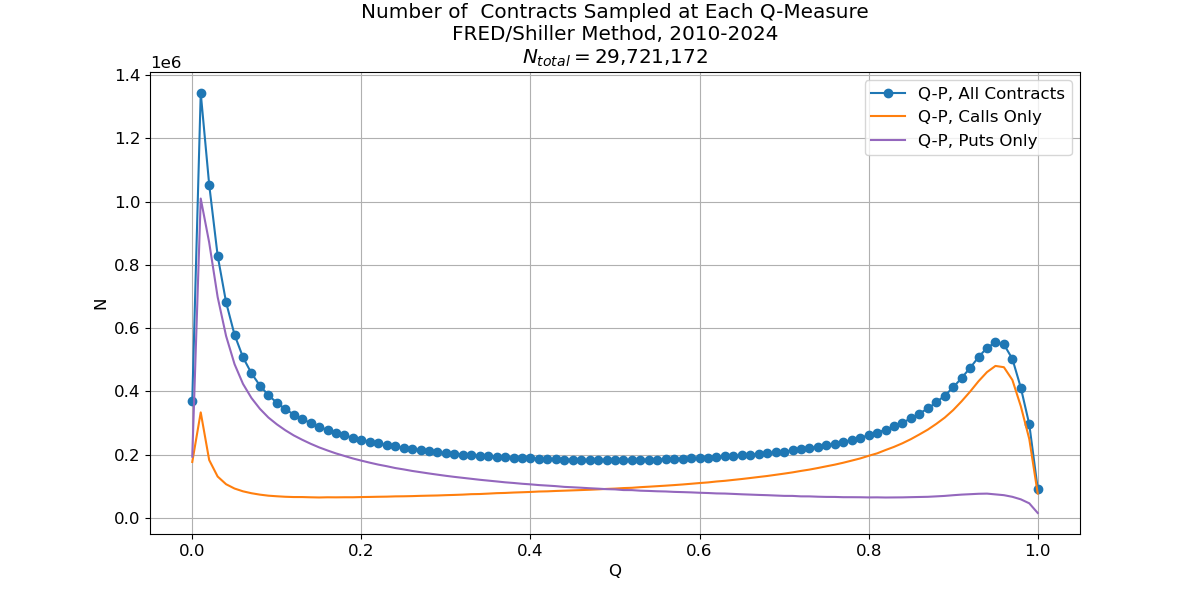
\includegraphics[width=1\textwidth]{fred_shiller_n_.png}
        \captionsetup{width=.5\linewidth}
        \caption{The number of samples in each $Q$ bin for the FRED/Shiller method, from which $P$ is computed.}
        \label{fig:fred_shiller_n}
    \end{figure}

    \begin{figure}[btp]
        \centering
        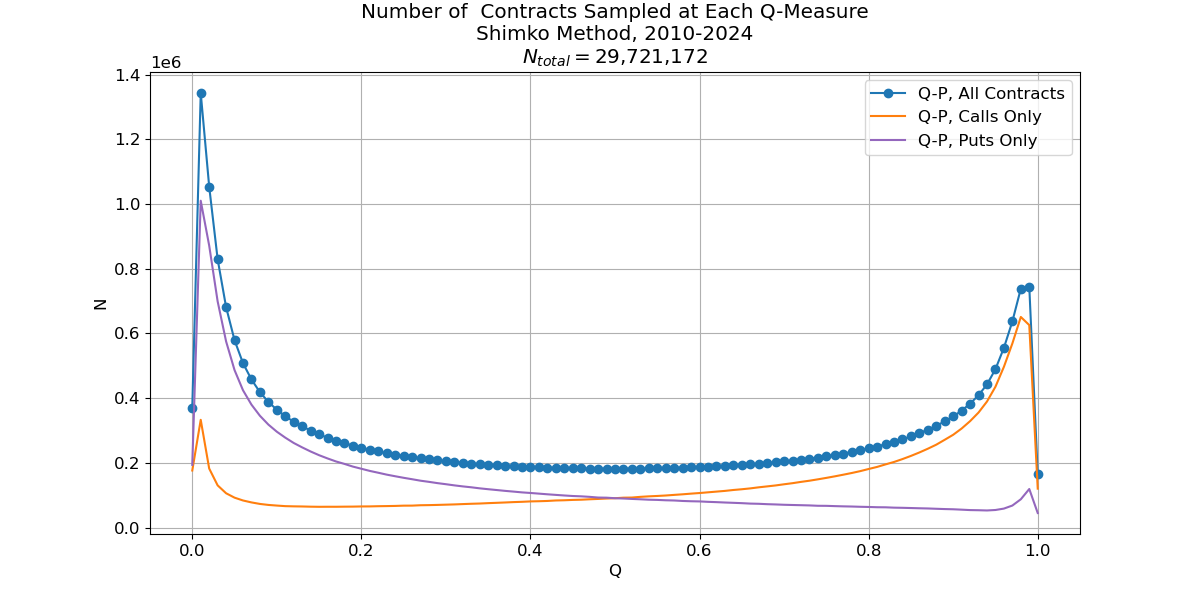
\includegraphics[width=1\textwidth]{shimko_n_.png}
        \captionsetup{width=.5\linewidth}
        \caption{The number of samples in each $Q$ bin for the Shimko method, from which $P$ is computed. These values are similar to those in Fig. \ref{fig:fred_shiller_n}, but with a sharper peak at high $Q$ values.}
        \label{fig:shimko_n}
    \end{figure}

  \subsection{Detrending}
    In addition to computing $P$-measures from binned expiry data, we also examined the effect of drift on the relationship between $Q$ and $P$. The stock market's tendency to drift upward over time is a commonly observed historical behavior that may influence the extent to which $Q$ over- or underestimates $P$. This is because the pricing kernel $m$ (also called the "stochastic discount factor") represents the $P$-probabilities investors currently expect for an asset, modified by their risk premia. Formally, $m$, $Q$, and $P$ are related through the equation:

    \begin{align}
      m = {\rm e}^{-r T} \frac{dQ}{dP}
    \end{align}

    If $Q$ and $P$ are related through investors' risk preferences and historical $P$ shows a consistent uptrend, then it is not unreasonable to consider whether the probability risk premium--denoted by $Q-P$ and implied by options prices--accounts for the historical market uptrend. By subtracting the average upward SPX drift and reconstructing the SPX price at expiry, we obtained the detrended SPX expiry price $\hat{S}_f$ and used it to compute $\hat{P}$, the real-world probability of expiring ITM under the detrended market process.

    Since market participants only ever have access to present and past data, we computed the expanding mean log-return $\mu_t$ at daily intervals, with the left side anchored at Yahoo Finance's earliest available date for SPX--back in the 1920's-- and the right side rolling at date $t$. For each of the roughly 30 million contract-days, we reconstructed the price series as $\hat{S}_t$ by subtracting $\mu_t$ from the daily log-returns and summing the resulting, detrended returns from entry to expiry:

    \begin{align}
      \hat{S}_f = S_t \exp{
        \left(\displaystyle \sum_{\tau=t+1}^{T}{
          \ln{
            \left(\frac{S_\tau}{S_{\tau-1}}\right)
          } - \mu_\tau
        }\right)
      }
    \end{align}

    For standard index options with their AM-settlements, we modified this by computing a second trend average $\mu_t^\ast$ representing the mean overnight log-return, measured from one day's closing price to the next day's opening price. We then replaced the final value $\mu_T$ with the overnight average $\mu_T^\ast$ to detrend the underlying for standard contracts:

    \begin{align}
      \hat{S}_f = S_t \exp{
        \left(
          \ln{
            \left(\frac{S_T}{S_{T-1}}\right)
          } - \mu_T^\ast +
          \displaystyle \sum_{\tau=t+1}^{T-1}{
          \ln{
            \left(\frac{S_\tau}{S_{\tau-1}}\right)
          } - \mu_\tau
        }\right)
      }
    \end{align}

    These detrended final states $S_f^\ast$ produced new probabilities $P^\ast$ without changing the risk-neutral probabilities $Q$, which derive from options prices at the entry date. Comparing $Q-P^\ast$ to $Q-P$ allowed us to measure the impact of historical market drift on probability risk premia.

\section{Results and Discussion}
    \subsection{Method Comparison on Real-World Underlying}
      Figures \ref{fig:fred_shiller_q_minus_p} and \ref{fig:shimko_q_minus_p} show the probability risk premia $Q-P$ produced via the FRED/Shiller and Shimko methods, respectively, plotted against $Q$ on the horizontal axis. The orange curves represent calls only; the purple curves show puts only; the blue curves show premia averaged over all contracts. The green and red shaded regions depict areas where the overall premia are positive and negative, respectively.

      According to these charts, call options consistently underestimate the probability of expiring ITM for virtually all values of $Q$--which roughly correlate with the more commonly used deltas that traders often refer to as a proxy for $Q$. The largest discrepancy occurs at strikes that are just slightly OTM, as represented by the orange curve's minimum value located at $Q\approx40\%$. This extremum shows that $Q$ can be as much as 25\% lower than $P$ for call options. By way of example, an average call option with a Prob(ITM) of 40\% (and a delta of roughly 0.4) will, in reality, expire in-the-money 65\% of the time.
      
      In contrast, puts consistently overestimate the probability of expiring ITM for virtually all values of $Q$, with the peak PRP occuring just slightly ITM at $Q\approx60\%$. This extremum shows that $Q$ can be up to 25\% \textit{higher} than $P$ for put options. In other words, an average put option with a Prob(ITM) of 60\% (and a delta of roughly 0.6) will, in reality, expire-in-the-money only 35\% of the time.
      
      Together, the PRPs for all contracts are generally positive OTM and negative ITM, approaching zero ATM. This means that, for OTM strikes, the probability risk premia from put options outweigh those of call options; the opposite is true for ITM strikes. One implication is that regime-agnostic trading strategies involving buying calls and selling puts may have a statistical edge on expiration day. In this, both the FRED/Shiller and Shimko methods produce agreeing results. The most notable difference between the two methods is that the probability risk premium from the FRED/Shiller method reaches zero slightly OTM, whereas the PRP obtained via Shimko's method reaches zero ATM, which suggests that Shimko's method may be a more balanced way of obtaining the $r$ and $q$ inputs for the Black-Scholes-Merton equation. 

      \begin{figure}[btp]
        \centering
        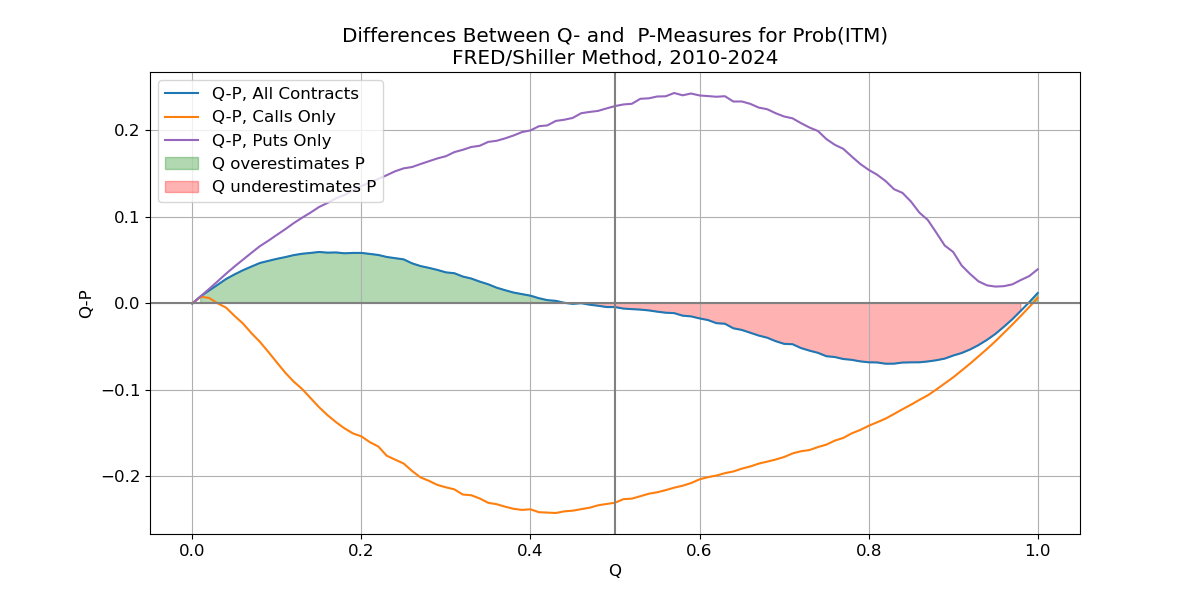
\includegraphics[width=1\textwidth]{fred_shiller_q_minus_p_.png}
        \captionsetup{width=.5\linewidth}
        \caption{Probability risk premia obtained via the FRED/Shiller method for calls (orange), puts (purple), and all contracts (blue) at each $Q$-measure bin. The green and red shaded areas depict positive and nengative premia, respectively. Notice how the premia for all contracts is slightly asymetrical, reaching zero just left of center, at roughly $Q=45\%$.}
        \label{fig:fred_shiller_q_minus_p}
      \end{figure}

      \begin{figure}[btp]
        \centering
        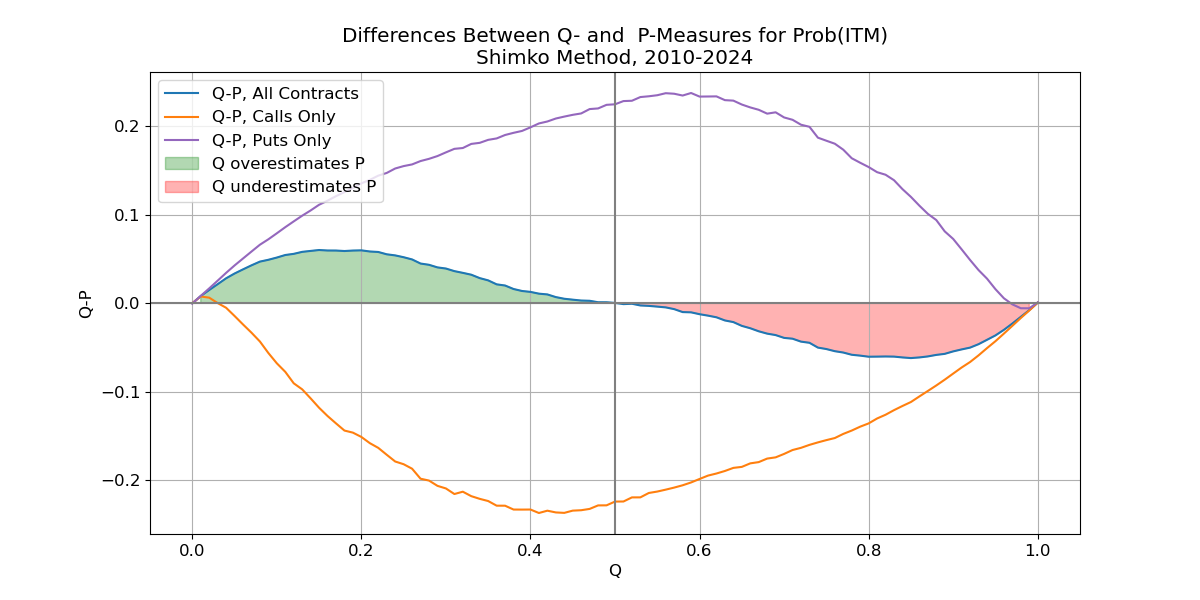
\includegraphics[width=1\textwidth]{shimko_q_minus_p_.png}
        \captionsetup{width=.5\linewidth}
        \caption{Probability risk premia obtained via the Shimko method for calls (orange), puts (purple), and all contracts (blue) at each $Q$-measure bin. Unlike that of the FRED/Shiller method, the blue curve in this graph reaches zero at-the-money, where $Q=50\%$. This suggests that the Shimko method is a more balanced approach to deriving inputs for the Black-Scholes-Merton equation.}
        \label{fig:shimko_q_minus_p}
      \end{figure}

    \subsection{Method Comparison on Detrended Underlying}
      Detrending SPX returns allows us to examine the probability risk premium in a world where stock market prices are generally stationary--at least throughout the lifetime of an option contract. By comparing PRP under a detrended stochastic process to the PRP generated by real-world prices, we can determine the extent to which SPX's historical uptrend influences the PRP. Figures \ref{fig:fred_shiller_q_minus_p_detrended} and \ref{fig:shimko_q_minus_p_detrended} show the probability risk premia $Q-P$ produced via the FRED/Shiller and Shimko methods, respectively, under the detrended stock process.

      Whereas the real-world PRP is positive for puts and negative for calls, the detrended PRP is positive for both OTM puts and calls, but is negative for ITM puts and calls. The FRED/Shiller and Shimko methods both generate PRP curves that are, in aggregate for all contracts, symmetrical about the $Q=50\%$ vertical line. Furthermore, call PRPs generally follow the S-shaped pattern of the puts, but with a negative offset that converges to zero at either extremum. This finding suggests that, while the historical market uptrend may account for some of the probability risk premia for calls and puts, it does not fully explain the premia priced into OTM puts or ITM calls; meanwhile, it seems to overexplain the premia priced into OTM calls and ITM puts.

      \begin{figure}[btp]
        \centering
        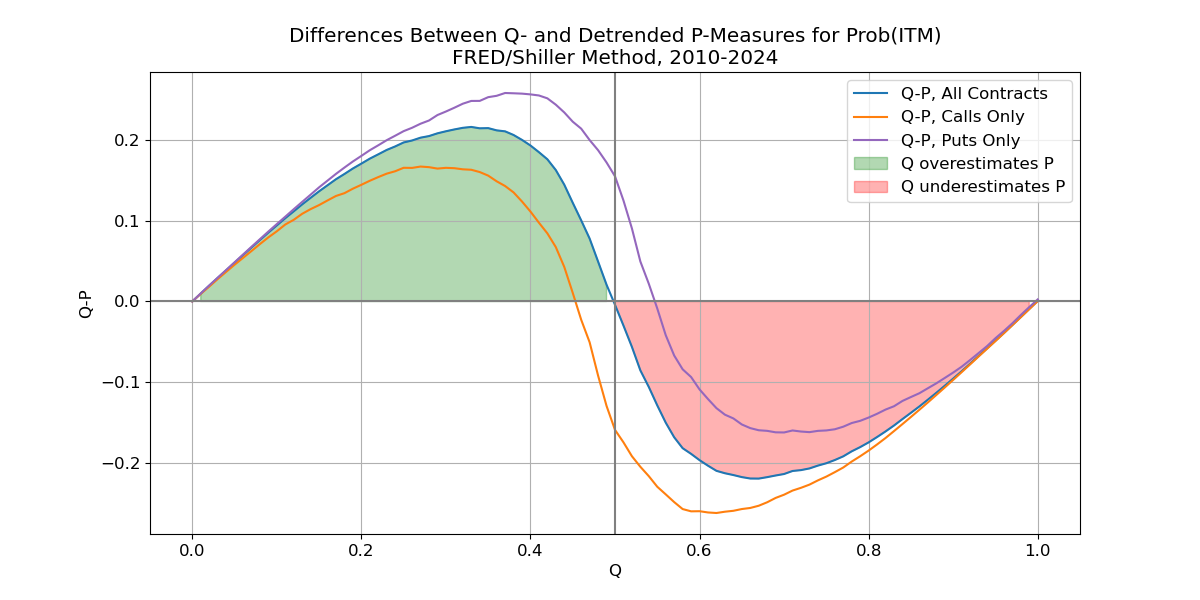
\includegraphics[width=1\textwidth]{fred_shiller_q_minus_p_detrended.png}
        \captionsetup{width=.5\linewidth}
        \caption{Probability risk premia under the detrended SPX process, obtained via the FRED/Shiller method. In comparison to the non-detrended version of this graph in Fig. \ref{fig:fred_shiller_q_minus_p}, the blue curve here is symmetrical and reaches zero at $Q=50\%$. Strangely, the sign of $Q-P$ for OTM calls and ITM puts is flipped, resulting in S-shaped curves.}
        \label{fig:fred_shiller_q_minus_p_detrended}
      \end{figure}

      \begin{figure}[btp]
        \centering
        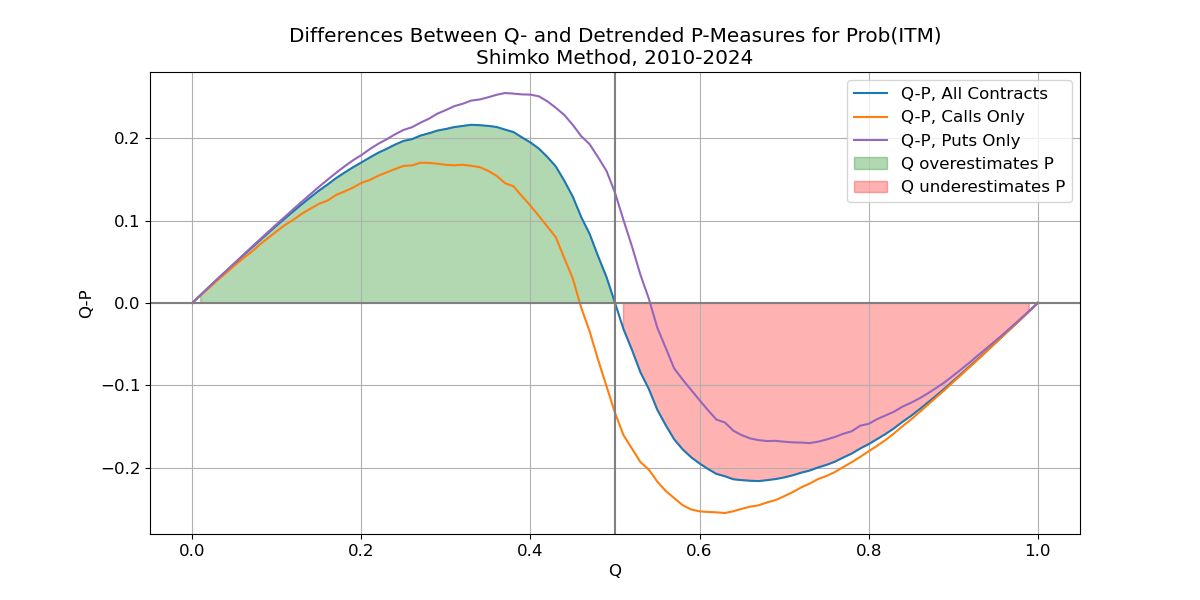
\includegraphics[width=1\textwidth]{shimko_q_minus_p_detrended.png}
        \captionsetup{width=.5\linewidth}
        \caption{Probability risk premia under the detrended SPX process, obtained via the Shimko method. These curves are difficult to distinguish from those of the detrended FRED/Shiller method.}
        \label{fig:shimko_q_minus_p_detrended}
      \end{figure}

    \subsection{Differences Between FRED/Shiller and Shimko Probability Risk Premium}
      Since the FRED/Shiller method relies on yield curve data and historical SPX dividends for obtaining the $r_f$ and $q$ inputs to the Black-Scholes-Merton equations, it represents an idealized world in which traders earn published yields and dividends remain constant. In reality, trading friction in bond markets and changing dividends produce widely varying costs-of-carry. Shimko's method addresses this reality by using a no-arbitrage (via put-call parity) argument to extract the $r_f$ and $q$ values implied by options prices.

      We compared the probability risk premia for the Shimko and FRED/Shiller methods in Figure \ref{fig:shimko_minus_fred_shiller_q} by subtracting one from the other with respect to $Q$. The top section shows that, overall, Shimko's method produces a PRP up to 1\% higher across most $Q$-values. The middle section reveals that this is true also for calls only. The bottom section shows that Shimko's method produces a slightly lower PRP for put options for most $Q$-values, with wider differences at high $Q$-values. This suggests that probability risk premia implied by options prices are slightly higher for calls and slightly lower for puts when compared to the idealized world assumed by the FRED/Shiller method.

      Detrending underlying returns causes the Shimko and FRED/Shiller methods to converge at extreme $Q$-values, but with greater divergence at-the-money. Figure \ref{fig:shimko_minus_fred_shiller_q_detrended} shows that Shimko's method reveals a decisively higher PRP for ATM calls and lower PRP for ATM puts. Overall, Shimko's method tends to produce higher risk premia under both historical and detrended returns.

      \begin{figure}[btp]
        \centering
        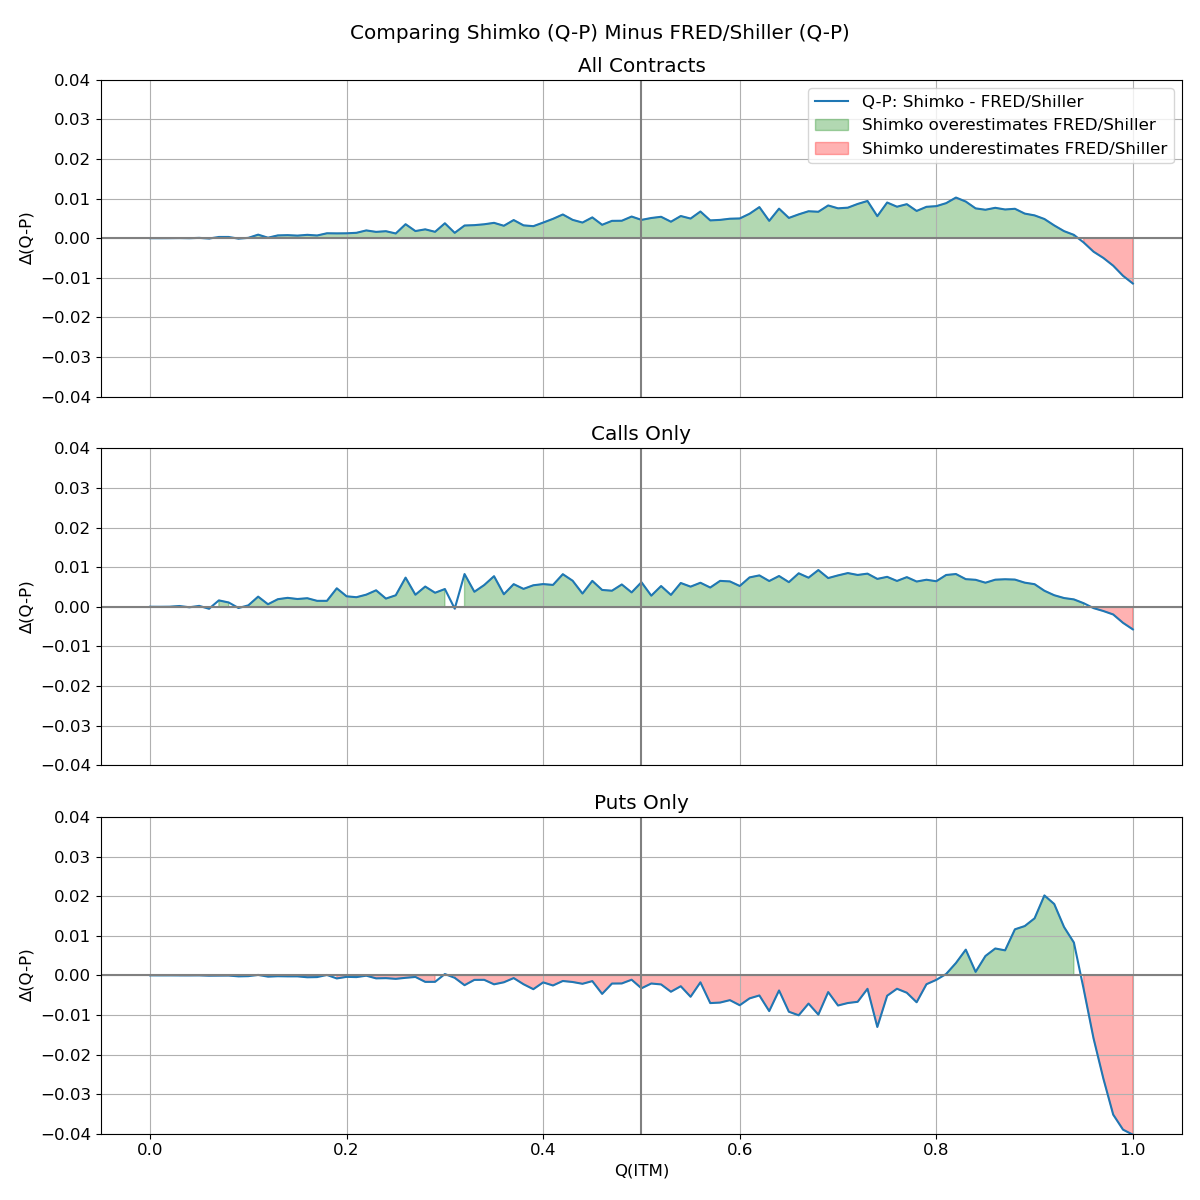
\includegraphics[width=1\textwidth]{shimko_minus_fred_shiller_q_.png}
        \captionsetup{width=.5\linewidth}
        \caption{Differences between probability risk premia for the Shimko method and for the FRED/Shiller method, plotted across each $Q$-bin. Green regions depict the Shimko probability risk premia exceeding that of the FRED/Shiller method; red regions show a relative defecit. For most $Q$-measures, the Shimko method produces a higher PRP for calls and a lower PRP for puts. At extreme ITM $Q$-measures, Shimko shows a slightly lower PRP calls and an exceedingly lower PRP for puts.}
        \label{fig:shimko_minus_fred_shiller_q}
      \end{figure}

      \begin{figure}[btp]
        \centering
        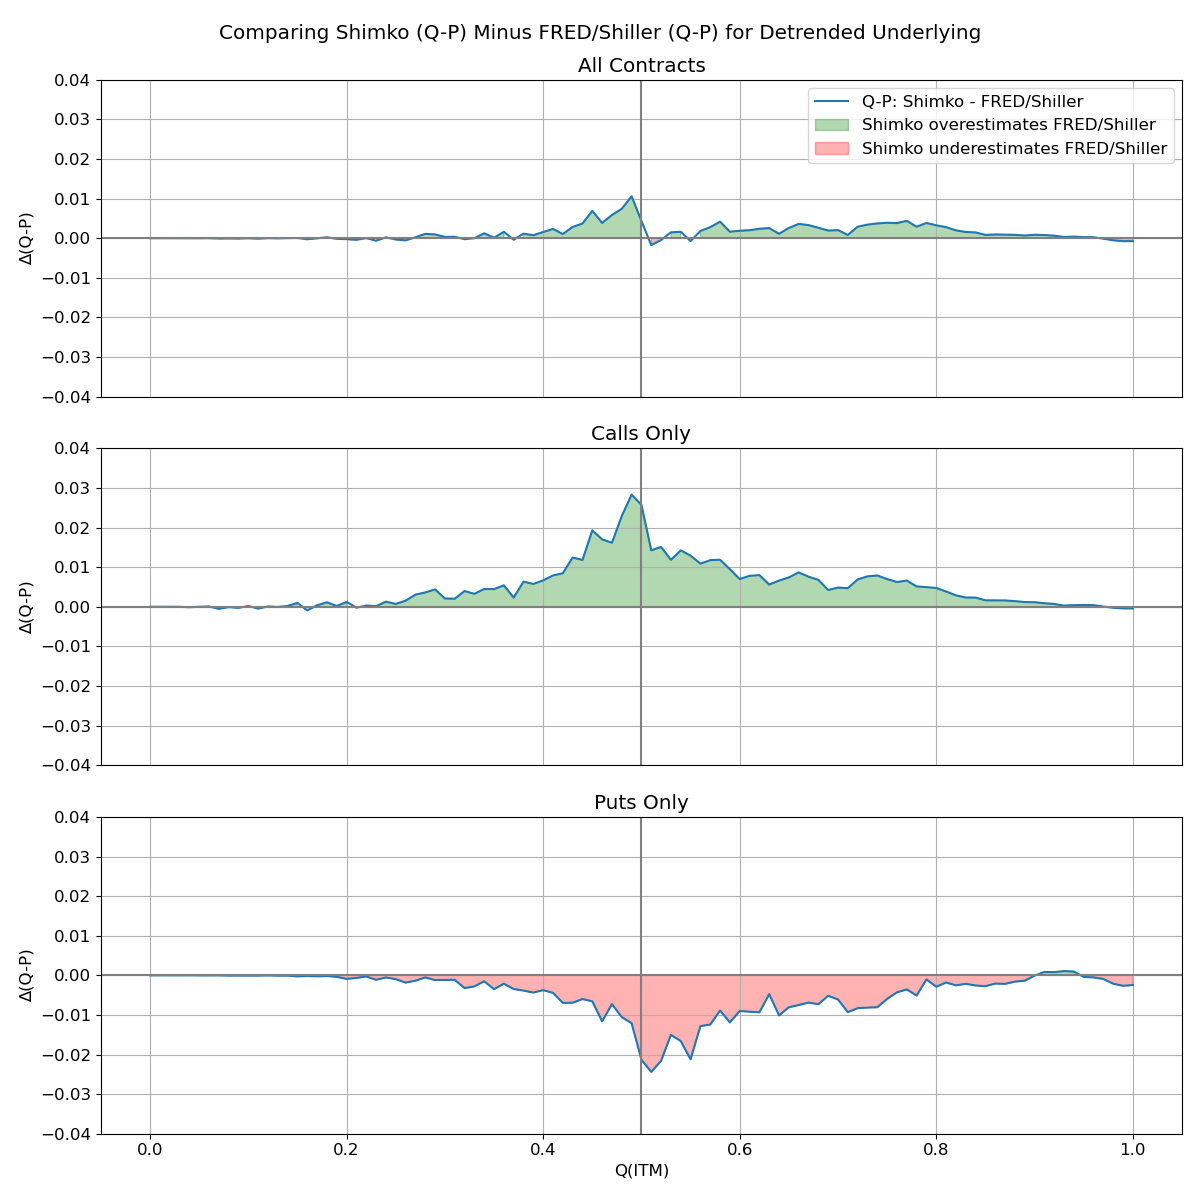
\includegraphics[width=1\textwidth]{shimko_minus_fred_shiller_q_detrended.png}
        \captionsetup{width=.5\linewidth}
        \caption{Differences between probability risk premia under the detrended SPX process for the Shimko method and for the FRED/Shiller method, plotted across each $Q$-bin. For most $Q$-measures, the Shimko method still produces a higher PRP for calls and a lower PRP for puts, however the distribution of these premia is different under the detrended process. Here, the largest premia occur at-the-money and are more balanced about the $Q=50\%$ vertical line.}
        \label{fig:shimko_minus_fred_shiller_q_detrended}
      \end{figure}


\section{Conclusion and Future Work}
  We compared risk-neutral probabilities to real-world outcomes for roughly 30 million option contract-days ranging from January 2010 through December 2024. We found that call options exhibited negative probability risk premia on average, indicating that they have historically underestimated the real-world probability of expiring in-the-money. The opposite is true for put options, which exhibited a generally positive PRP resulting in an overestimate of expiring ITM. For both calls and puts, the greatest discrepancies between risk-neutral and real-world probabilities occured near-the-money, between deltas of roughly 0.4 and 0.6. We found that detrending the underlying SPX index did not sufficiently neutralize the risk premia for OTM puts or ITM calls, suggesting that the historical market trend does not account for the observed risk-premia.
  
  In addition to comparing risk-neutral and real-world probabilities, we also compared two different methods -- the FRED/Shiller and Shimko methods -- for obtaining the risk-free rate and continuous dividend yield inputs to the Black-Scholes-Merton equations. We found that Shimko's method produces slightly higher risk premia (between 0\% and 1\%) than the FRED/Shiller method, on average.

  In assessing the impact of the historical market trend on probability risk premia, we simply subtracted the drift term $\mu_t$ from daily log-returns. However, $Q$-probabilities assume an equivalent martingale measure that discounts future states according to the risk-free rate $r$. Accordingly, future efforts should re-examine the $Q$-dependent probability risk premia after subtracting $\mu_t-r$ from daily log-returns.
  
  In applying the FRED/Shiller method, we assumed that the most recent quarterly dividend yield data is relevant for pricing options contracts, but real yields change over time and future yields may be different from the 12-month trailing yields posted last quarter. To rectifiy this, future research could apply a predictive model to S\&P 500 yields--such as a linear extrapolation--to better capture the market's anticipated dividend that is baked into options prices.
  
  Finally, our analysis focused on the discrepancy between risk-neutral probabilities and historical realized probabilities over the 15-year window of 2010-2024. This period witnessed a long bull market, a few minor pullbacks, the COVID market crash of 2020, and the 2022 bear market, but did not include the 2008 financial crisis nor the 2000 dot-com bubble. The overwhelming trend during our selected period was bullish. Future reasearch should explore how the probability risk premium behaves in different market regimes, as this information will enable traders to make better informed options pricing decisions in the short-term.

\bibliographystyle{elsarticle-harv} 
\bibliography{references}

\end{document}

\endinput
%%
%% End of file
